\documentclass{beamer}
\usepackage[utf8]{inputenc}
\usepackage{default}
\usepackage{listings}
\usepackage{relsize}
\usepackage{graphicx}

\mode<presentation>{ \usetheme{Singapore} }
\title{ Palestra com nome engraçadinho pra chamar gente }
\subtitle{ A construção do Caos }
\author{ Tomaz Canabrava }

\AtBeginSection[]
{
   \begin{frame}
       \frametitle{Outline}
       \tableofcontents[currentsection]
   \end{frame}
}

\begin{document}
\begin{frame} \titlepage \end{frame}

\section{Pré história}

\begin{frame} \frametitle{1940}
    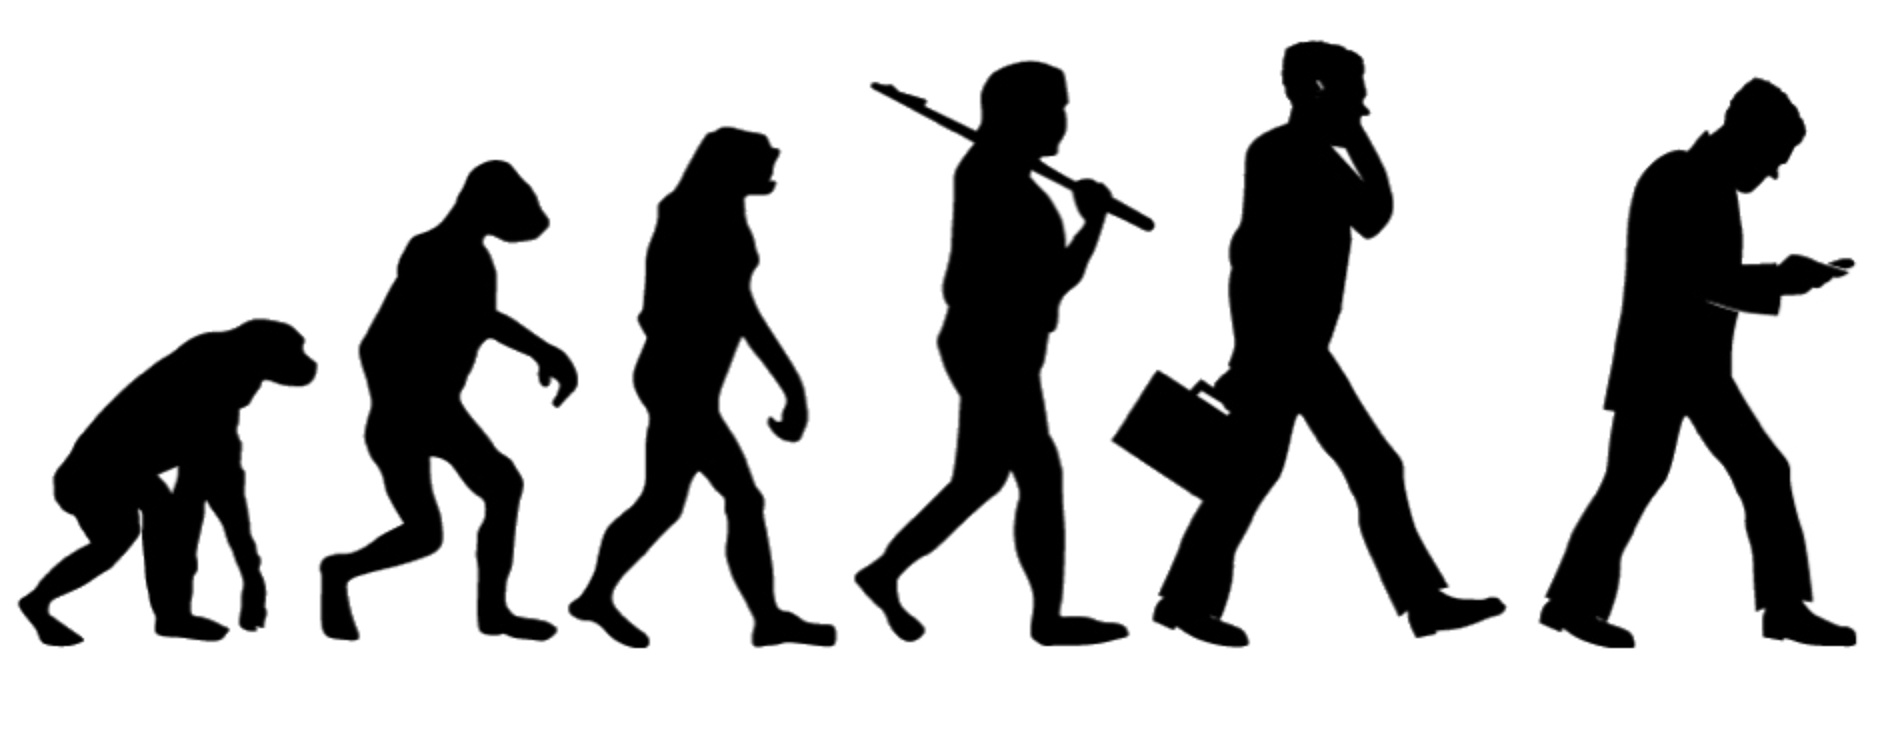
\includegraphics[width=300px]{images/evolution}
\end{frame}

\begin{frame} \frametitle{Invenções Pré-históricas}
    \begin{itemize}
     \item Fogo
     \item Roda
     \item Imprensa
     \pause
     \item Eniac
    \end{itemize}
\end{frame}

\begin{frame} \frametitle{Eniac}
    
\includegraphics[width=300px]{images/eniac}
\end{frame}

\begin{frame} \frametitle{Eniac em 1940}
    \begin{columns}
    \column{0.5\textwidth}
    \begin{itemize}
        \item Base 10
        \pause
        \item 5000 calculos por segundo
        \pause
        \item 5 Milhões pontos de solda manuais
        \pause
        \item 150kw de energia
        \pause
        \item Não cabia no seu bolso.
    \end{itemize}
    \end{columns}
\end{frame}

\begin{frame} \frametitle{Uma olhada em 150kw}
    \begin{itemize}
    \item 3750 lampadas de 40w
    \item Carregar 150 Androids por um Ano
    \item Um Laser Militar (Ainda em Construção)
    \end{itemize}
\end{frame}

\begin{frame} \frametitle{IBM}
    \begin{columns}
        \column{0.5\textwidth}
        ''I think there is a world market for about five computers''

        Thomas J Watson
        \pause
        \column{0.5\textwidth}
        ''Eu acho que existe um mercado mundial para uns cinco computadores''
    \end{columns}
\end{frame}

\begin{frame} \frametitle{1960 e MainFrames}

\end{frame}

\end{document}
